% ============================================================
%  TERM PROJECT – PROPOSAL (template)
%  Databases · THGA Bochum
%
%  How to use:
%    1. Copy this folder into your own repository.
%    2. Replace every  <<< ... >>>  placeholder with your content.
%    3. Build with  `make`  (see the Makefile / README).
%    4. Send the resulting PDF to the lecturer and wait for approval.
% ============================================================
\documentclass[11pt,a4paper]{article}

\usepackage{thga-db}
\usepackage{caption}   % enables \captionof inside minipages

% ----- Fill in your metadata -------------------------------
\renewcommand{\thgaKurs}{Databases}
\renewcommand{\thgaDatum}{Summer Term 2026}
\newcommand{\authorName}{Meriem Kaddoum}
\newcommand{\projectTitle}{Pet Adoption Management System}

\begin{document}
\thispagestyle{empty}
\thgaTitel{Term Project – Proposal}{\projectTitle}

\begin{infobox}
\textbf{Author:} \authorName \\
\textbf{Module:} Introduction to Database Management Systems · THGA Bochum \\
\textbf{Submitted to:} Stephan Bökelmann · \href{mailto:sboekelmann@ep1.rub.de}{sboekelmann@ep1.rub.de} \\
\textbf{Target size:} about 6 pages
\end{infobox}

\begin{infobox}
\textbf{Every figure must be explained in the running text.} A figure never
stands on its own: refer to it by number and say what it shows -- e.g.
``Figure~\ref{fig:er} shows the ER model of \dots''.

Every figure below is \texttt{example-figure.jpg}, a dummy image shipped with
this template. Photograph or scan your own sketch, drop the file next to
\texttt{proposal.tex}, and point \texttt{\textbackslash includegraphics} at it:
\begin{quote}
\texttt{\textbackslash includegraphics[width=0.85\textbackslash linewidth]\{er-sketch.jpg\}}
\end{quote}
The \texttt{width} option scales the image to a fraction of the text width; the
file extension may be omitted. Keep the \texttt{\textbackslash caption} and the
\texttt{\textbackslash label} as they are.
\end{infobox}

% ============================================================
\section{Application domain and motivation}
% ============================================================

The proposed application is a \textbf{Pet Adoption System}, a database-backed system
designed to support animal shelters in managing pets, adopters and adoption
processes. Many small and medium-sized shelters still rely on spreadsheets or
paper records, making it difficult to maintain accurate information about
available pets, adoption history and adopter data.

The system is mainly intended for shelter employees and administrators. They can
register new pets, update pet information, manage adopter records and record
completed adoptions. Visitors benefit from an always up-to-date overview of
available animals.

\textbf{Usage scenario 1:}
A family visits the shelter looking for a dog. The employee searches the
database for all available dogs, filters them by age and breed, and creates a
new adoption record after the family chooses a pet.

\textbf{Usage scenario 2:}
A previously adopted pet is returned to the shelter. The employee updates the
adoption status and marks the pet as available again so that it can be adopted
by another family.

% ============================================================
\section{Data model -- ER sketch}
% ============================================================

\begin{figure}[ht]
  \centering
<<<<<<< HEAD
  % Swap example-figure.jpg for your own file, e.g. er-sketch.jpg
  % (a photographed hand drawing is fine).
  \includegraphics[width=0.85\linewidth]{example-figure.jpg}
  \caption{ER sketch of the <<< domain >>> data model: entity types, key
=======
  % Replace the placeholder with: \includegraphics[width=0.85\linewidth]{er-sketch.jpg}
  \includegraphics[width=0.7\linewidth]{er-sketch.jpg}
  \caption{ER sketch of the Pet Adoption System data model: entity types, key
>>>>>>> 7f17527 (Add completed project proposal)
  attributes, relationships and cardinalities (at least one N:M).}
  \label{fig:er}
\end{figure}

Figure~\ref{fig:er} shows the ER model of the Pet Adoption System. The main
entities are \textbf{Shelter}, \textbf{Pet}, \textbf{Adopter} and
\textbf{Adoption}. A shelter manages many pets (1:N), while an adopter can have
multiple adoption records over time (1:N). The Adoption entity stores the
adoption date and status and resolves the many-to-many relationship between
pets and adopters.

% ============================================================
\section{From model to schema}
% ============================================================

The relational schema is derived directly from the ER model. Each table has a
single primary key, while relationships between entities are represented by
foreign keys. The adoption process is stored in a separate table, which resolves
the many-to-many relationship between pets and adopters.

\begin{itemize}
\item \texttt{Shelter}(\underline{shelter\_id}, name, address, phone)

\item \texttt{Pet}(\underline{pet\_id}, name, species, breed, age, gender,
status, \emph{shelter\_id})

\item \texttt{Adopter}(\underline{adopter\_id}, first\_name, last\_name,
email, phone)

\item \texttt{Adoption}(\underline{adoption\_id},
adoption\_date, status,
\emph{pet\_id},
\emph{adopter\_id})

\textbf{Normalisation.}
The database schema satisfies the Third Normal Form (3NF). Every table stores
information about exactly one entity, and each non-key attribute depends only on
the primary key of its own table. Repeated information is avoided by using
foreign keys instead of duplicating data. The Adoption table resolves the
many-to-many relationship between pets and adopters without introducing
redundancy or update anomalies.

\end{itemize}


% ============================================================
\section{API design}
% ============================================================

The application provides a REST API implemented with FastAPI. Read endpoints are
available for retrieving pets and adoption statistics, while write endpoints are
protected by an X-API-Key. The API communicates directly with the PostgreSQL
database and is the only component allowed to access it. The frontend interacts
with the system exclusively through these endpoints.

\renewcommand{\arraystretch}{1.2}
\begin{tabularx}{\linewidth}{@{}p{2cm}p{4cm}X@{}}
\toprule
\textbf{Method} & \textbf{Path} & \textbf{Purpose} \\
\midrule
\texttt{GET}  & \texttt{/pets} &
Returns all available pets together with the shelter information (JOIN between
Pet and Shelter). \\

\texttt{GET} & \texttt{/adoptions/statistics} &
Returns the number of successful adoptions grouped by species
(aggregation using COUNT and GROUP BY). \\

\texttt{GET} & \texttt{/adopters/\{id\}/adoptions} &
Returns all adoptions of one adopter (JOIN between Adopter, Adoption and Pet). \\

\texttt{POST} & \texttt{/pets} &
Creates a new pet record (requires X-API-Key). \\

\texttt{POST} & \texttt{/adoptions} &
Creates a new adoption record and updates the pet status
(requires X-API-Key). \\

\texttt{PUT} & \texttt{/pets/\{id\}} &
Updates pet information such as status or age
(requires X-API-Key). \\

\texttt{DELETE} & \texttt{/pets/\{id\}} &
Deletes a pet that has never been adopted
(requires X-API-Key). \\
\bottomrule
\end{tabularx}

% ============================================================
\section{Frontend prototype (hand sketches)}
% ============================================================

The frontend will be implemented using Python and Tkinter because it is simple,
lightweight and integrates well with FastAPI. At startup, the application
displays a connection dialog where the user enters the API URL and the
X-API-Key. After a successful connection, the main window displays all available
pets retrieved from the backend.

Users can open a detail form to register new pets or update existing records.
Another screen is used to create adoption records, while a statistics screen
shows the number of successful adoptions grouped by species. All communication
between the frontend and the database is performed through the REST API.

% Each \includegraphics below still points at the dummy example-figure.jpg.
% Swap in your own file per screen, e.g. {fe-connect.jpg}, and keep the \captionof.
\begin{figure}[ht]
\centering
\begin{minipage}[t]{0.47\linewidth}\centering
<<<<<<< HEAD
  \includegraphics[width=\linewidth]{example-figure.jpg}
=======
\includegraphics[width=\linewidth,height=3.5cm,keepaspectratio]{connect.png}
>>>>>>> 7f17527 (Add completed project proposal)
  \captionof{figure}{Startup connection dialog: API URL + X-API-Key.}
  \label{fig:fe-connect}
\end{minipage}\hfill
\begin{minipage}[t]{0.47\linewidth}\centering
<<<<<<< HEAD
  \includegraphics[width=\linewidth]{example-figure.jpg}
  \captionof{figure}{Main screen: <<< list/table, calls \texttt{GET /<<<…>>>} >>>.}
=======
  \includegraphics[width=\linewidth,height=3.5cm,keepaspectratio]{main.png}
  \captionof{figure}{Main screen: Pet overview showing all available pets, calls \texttt{GET /pets}.}
>>>>>>> 7f17527 (Add completed project proposal)
  \label{fig:fe-main}
\end{minipage}

\vspace{1em}

\begin{minipage}[t]{0.47\linewidth}\centering
<<<<<<< HEAD
  \includegraphics[width=\linewidth]{example-figure.jpg}
  \captionof{figure}{Detail form: <<< create/edit, calls \texttt{POST /<<<…>>>} >>>.}
  \label{fig:fe-detail}
\end{minipage}\hfill
\begin{minipage}[t]{0.47\linewidth}\centering
  \includegraphics[width=\linewidth]{example-figure.jpg}
  \captionof{figure}{<<< Second feature screen and the endpoint it calls >>>.}
=======
  \includegraphics[width=\linewidth,height=3.5cm,keepaspectratio]{form.png}
  \captionof{figure}{Detail form:Pet registration form, calls \texttt{POST /pets}.}
  \label{fig:fe-detail}
\end{minipage}\hfill
\begin{minipage}[t]{0.47\linewidth}\centering
  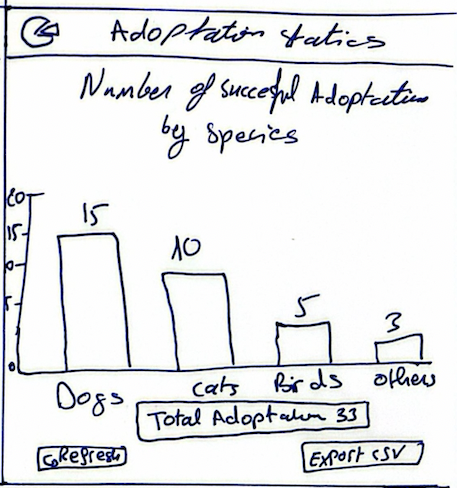
\includegraphics[width=\linewidth,height=3.5cm,keepaspectratio]{statistics.png}
  \captionof{figure}{Adoption statistics screen, calls \texttt{GET /adoptions/statistics}.}
>>>>>>> 7f17527 (Add completed project proposal)
  \label{fig:fe-second}
\end{minipage}
\end{figure}

Figure~\ref{fig:fe-connect} shows the connection dialog where the user enters
the API URL and the X-API-Key before accessing the application.
Figure~\ref{fig:fe-main} shows the main screen listing all available pets,
retrieved using \texttt{GET /pets}. Figure~\ref{fig:fe-detail} presents the form
used to register a new pet by calling \texttt{POST /pets}. Finally,
Figure~\ref{fig:fe-second} shows the statistics screen, which displays adoption
statistics retrieved through \texttt{GET /adoptions/statistics}.

% ============================================================
\section{Operation with Docker Compose}
% ============================================================

The application is deployed using Docker Compose and consists of two main
services: a PostgreSQL database and a FastAPI backend. The PostgreSQL container
stores all application data, while the FastAPI container provides the REST API
used by the frontend.

Database credentials, API keys and other configuration values are stored in a
separate \texttt{.env} file. This keeps sensitive information out of the source
code and allows different configurations for development and production.

On the lecture server, the backend is deployed by starting the Docker Compose
stack. Docker Compose automatically creates the required containers, connects
them through an internal network and ensures that the API can communicate with
the PostgreSQL database. The frontend accesses the backend through the API URL
configured in the connection dialog.

% ============================================================
\section{Scope, milestones and risks}
% ============================================================

\textbf{Scope.} The project consists of four database tables (Shelter, Pet, Adopter and
Adoption) and seven REST API endpoints. The endpoints support creating,
retrieving, updating and deleting records as well as providing adoption
statistics through an aggregation query.

\textbf{Milestones and schedule.} <<< Fill in the week and the estimated hours;
the hours should add up to roughly 40. >>>

\renewcommand{\arraystretch}{1.2}
\begin{tabularx}{\linewidth}{@{}p{1.4cm}Xp{1.8cm}@{}}
\toprule
\textbf{Week} & \textbf{Milestone} & \textbf{Est. hours} \\
\midrule
1 & Database schema, ER model and seed data completed & 8 \\

2--3 & FastAPI backend with CRUD endpoints, authentication using
X-API-Key and database integration & 12 \\

4--5 & Tkinter frontend connected to the API, Docker Compose setup and
application packaging & 10 \\

6 & Testing, bug fixing, documentation and project video & 10 \\
\bottomrule
\end{tabularx}

\textbf{Risks.} A possible risk is that communication between the frontend and backend may fail
because of incorrect API configuration or authentication settings. Another risk
is inconsistent database data caused by invalid foreign key references or
incorrect user input. Both risks will be addressed through automated tests and
input validation.
% ============================================================
\section{Acceptance criteria and testing}
% ============================================================

The project is considered complete when all planned database functions, REST API
endpoints and frontend features operate correctly. Each acceptance criterion can
be verified by automated or manual tests. Particular attention is given to
database integrity, API authentication and the communication between the
frontend and backend.

\textbf{Acceptance criteria.} The following criteria must be fulfilled before the project is considered
complete.
\begin{itemize}[topsep=2pt]
  \item Invalid records that violate database constraints are rejected and the API
returns an appropriate 4xx error response.

\item The endpoint \texttt{GET /adoptions/statistics} returns the correct
aggregated adoption statistics using SQL aggregation and grouping.

\item All write operations require a valid X-API-Key. Requests without a valid
key return HTTP status code 401 or 403.
\end{itemize}

\textbf{Test plan.} The project will be tested on the database, API and application levels using
both automated and manual tests.
\begin{itemize}[topsep=2pt]
  \item \textbf{Database:} Verification of primary keys, foreign keys, NOT NULL constraints and referential
integrity between all related tables.
  \item \textbf{API:} Endpoint tests using \texttt{pytest} together with FastAPI's
\texttt{TestClient}. Both successful requests and error cases such as invalid
input or missing authentication are verified using a separate test database.
  \item \textbf{Business rule:} Verify that adoption records cannot be created for pets that are already marked
as adopted and that requests without a valid X-API-Key are rejected.
\end{itemize}

\vspace{1em}
\begin{infobox}
\textbf{Effort budget:} the whole term project (system, documentation and video)
should fit into roughly \textbf{40\,h of work} over at most \textbf{2 months}.
Keep your scope within that budget.
\end{infobox}

\end{document}
